Below one can see the general framework of executables that this testing package generates to emulate
and decentralized system of 3 heterogeneous robots. Each robot is in its own namespace, allowing it
to have the same internal nodes as other robots as well as abstract away information that is only
pertinent to itself.

\begin{figure}[H]
  \centering
    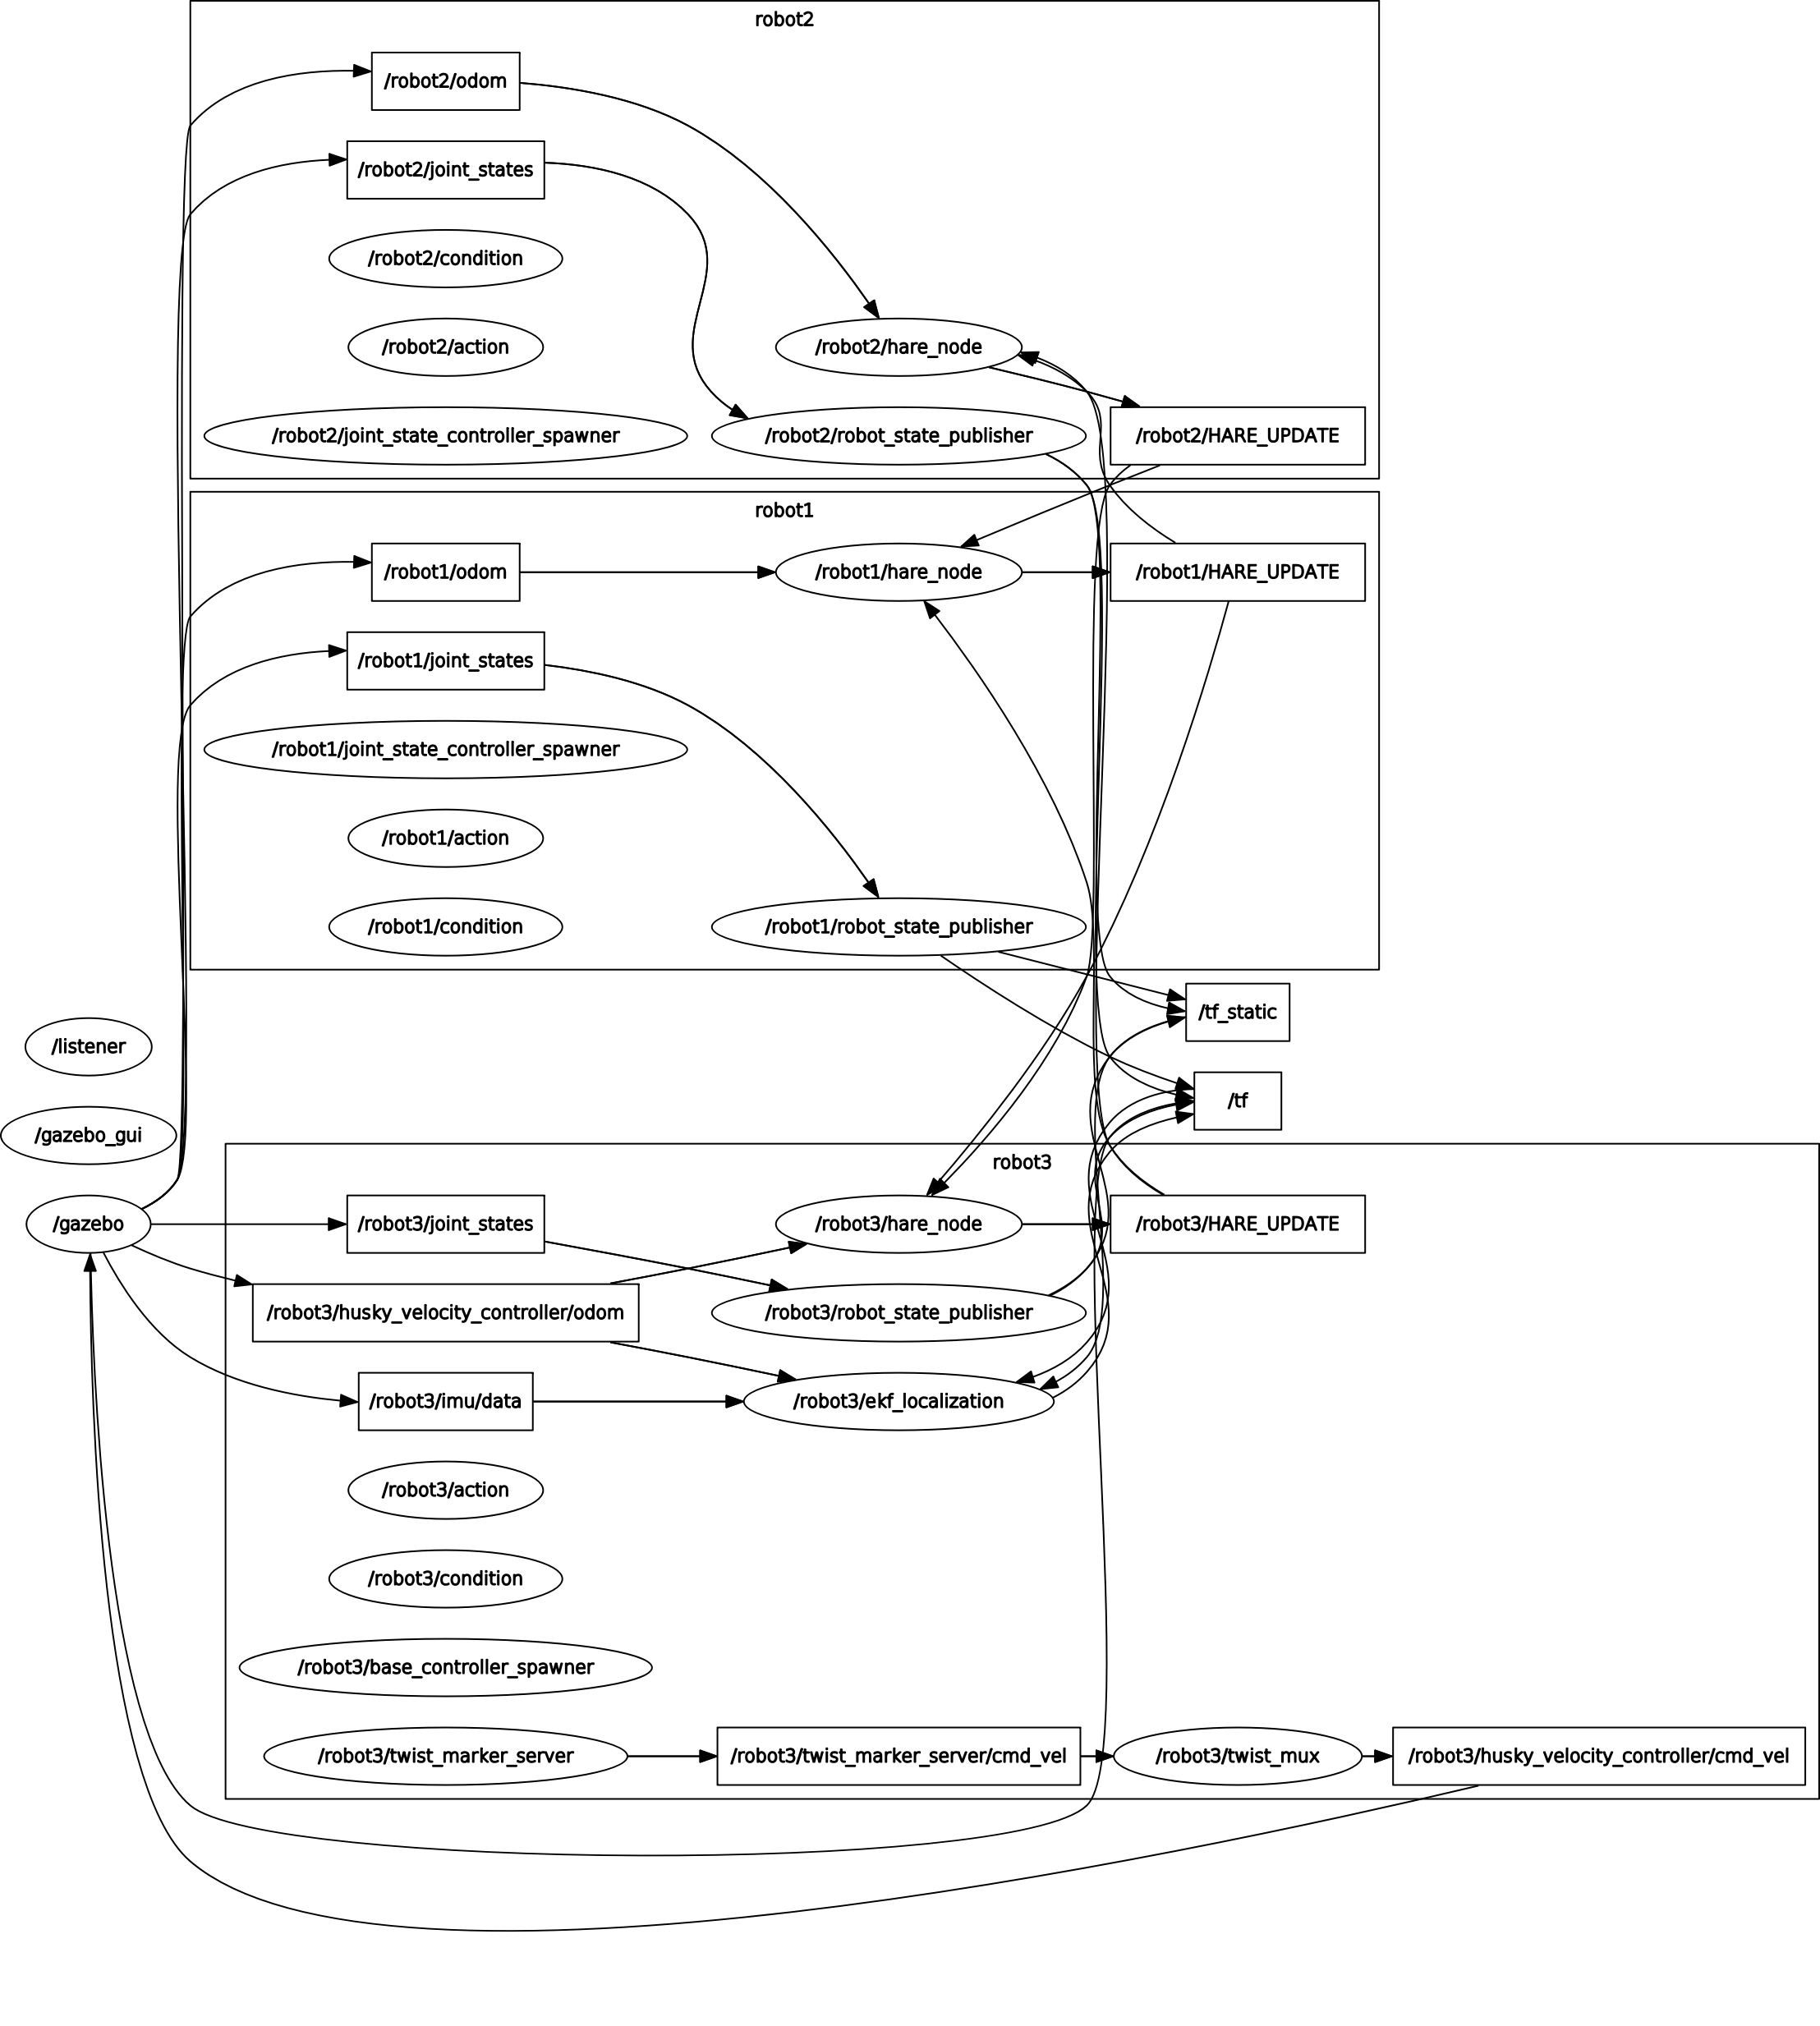
\includegraphics[width=0.95\textwidth]{rosgraph}
  \caption{RQT Graph of Peer-to-Peer ROS node organization}
  \label{fig:rosgraph}
\end{figure}

\subsection{Conclusion}

Over the course of this semester, even though a lot of problems were encountered
by this project, the learning experience was invaluable. Understanding a system like
ROS, especially being forced to understand it at a "deep C" level, opens a lot of doors
for my future research and ability to simulate ideas in a near real world environment.


\subsection{Future Work}

Primary future focus will be to get the testing framework wrapped up
for release as well as applying that completely finalized framework to
extensive heterogeneous multi-robot testing. Even though the testing framework
was not the overall goal of this research,
it turned out to be one of the strong suits of the project. Future work would certainly
include iteration on this framework to ensure that it is as easy as possible to
randomly generate maps as well as add any number of any kind of robot. The benefit
of doing this on Gazebo is the ability to emulate robotic agents much closer to the
real world representation than Unity, ARGoS, or any other open-source platform
capable of multi-robot simulation.

Another step would of course be iteration of the tested cooperation model on hardware.
This would require much more extraneous simulation to ensure that all edge cases are
covered. To properly do this, the testing framework would have to be iterated as
described above. Due to Gazebo not inherently supporting multimaster network architectures,
there is the possibility that a plugin or new simulation package would need to be
developed.

\subsection{Eventual Rejuvenation of Initial Goals}

What started as the basis of this research, was in the definition of attributes
to generalize robot software and hardware capabilities to optimally cooperate with
other heterogeneous robots. As this research was meant to strictly provide a basis
for heterogeneous task division and capability utilization, the model built on
top of it could take many forms. Fully fleshing out this system would be as simple as
having a reasonable usage for extensive robot capability information, really meaning that a
complex enough task would have to be derived and tested once the testing framework has been
completely solidified and ready for release. Before problems arose that required focus to
be redirected towards the testing framework that was implemented. To illustrate the thought
that went into attribute listing, the appendix has a set of tables that show where this
research is eventually headed.
